\chapter{実験結果}
\section{粘度 計測結果}
鋼球落下実験を行う試験溶液として,1wt.\%PAA溶液の製作を行った.この製作した溶液の粘度特性を確認し,先行研究\cite{ref:9}\cite{ref:10}における粘度特性と比較した.この比較を行うことで先行研究との粘度特性の違いを確認した.なお,この粘度計測は溶質が溶媒に十分に均一に溶解し,混合時に混入した気泡がおおむね消失する溶液製作1週間後に行った.それぞれの試料に対し,円錐回転子の回転数を変化させ,各5回計測を行いその平均を求めた.

PAA溶液の粘度計測を行った結果をFig.\ref{fig:PAA-vis}に示す.なお,縦軸は粘度,横軸はせん断速度を表す.第2章にても示したが,コーンロータの回転速度を変化させることにより,せん断速度を変化させた.

また,Iwamuro et al.\cite{ref:9}やShiratori et al.\cite{ref:10}の文献値も共に示した.ここで,粘度$\mu$はせん断速度$\dot{\gamma}$に対して,粘度定数 k[Pa・$s^n$],指数を用いると,the Power-law modelに従うものとすると,
\begin{eqnarray}
    \mu=k\times\dot{\gamma}^{n-1}
\end{eqnarray}
といった式で与えられる\cite{ref:1}.

\begin{figure}[h]
    \centering
    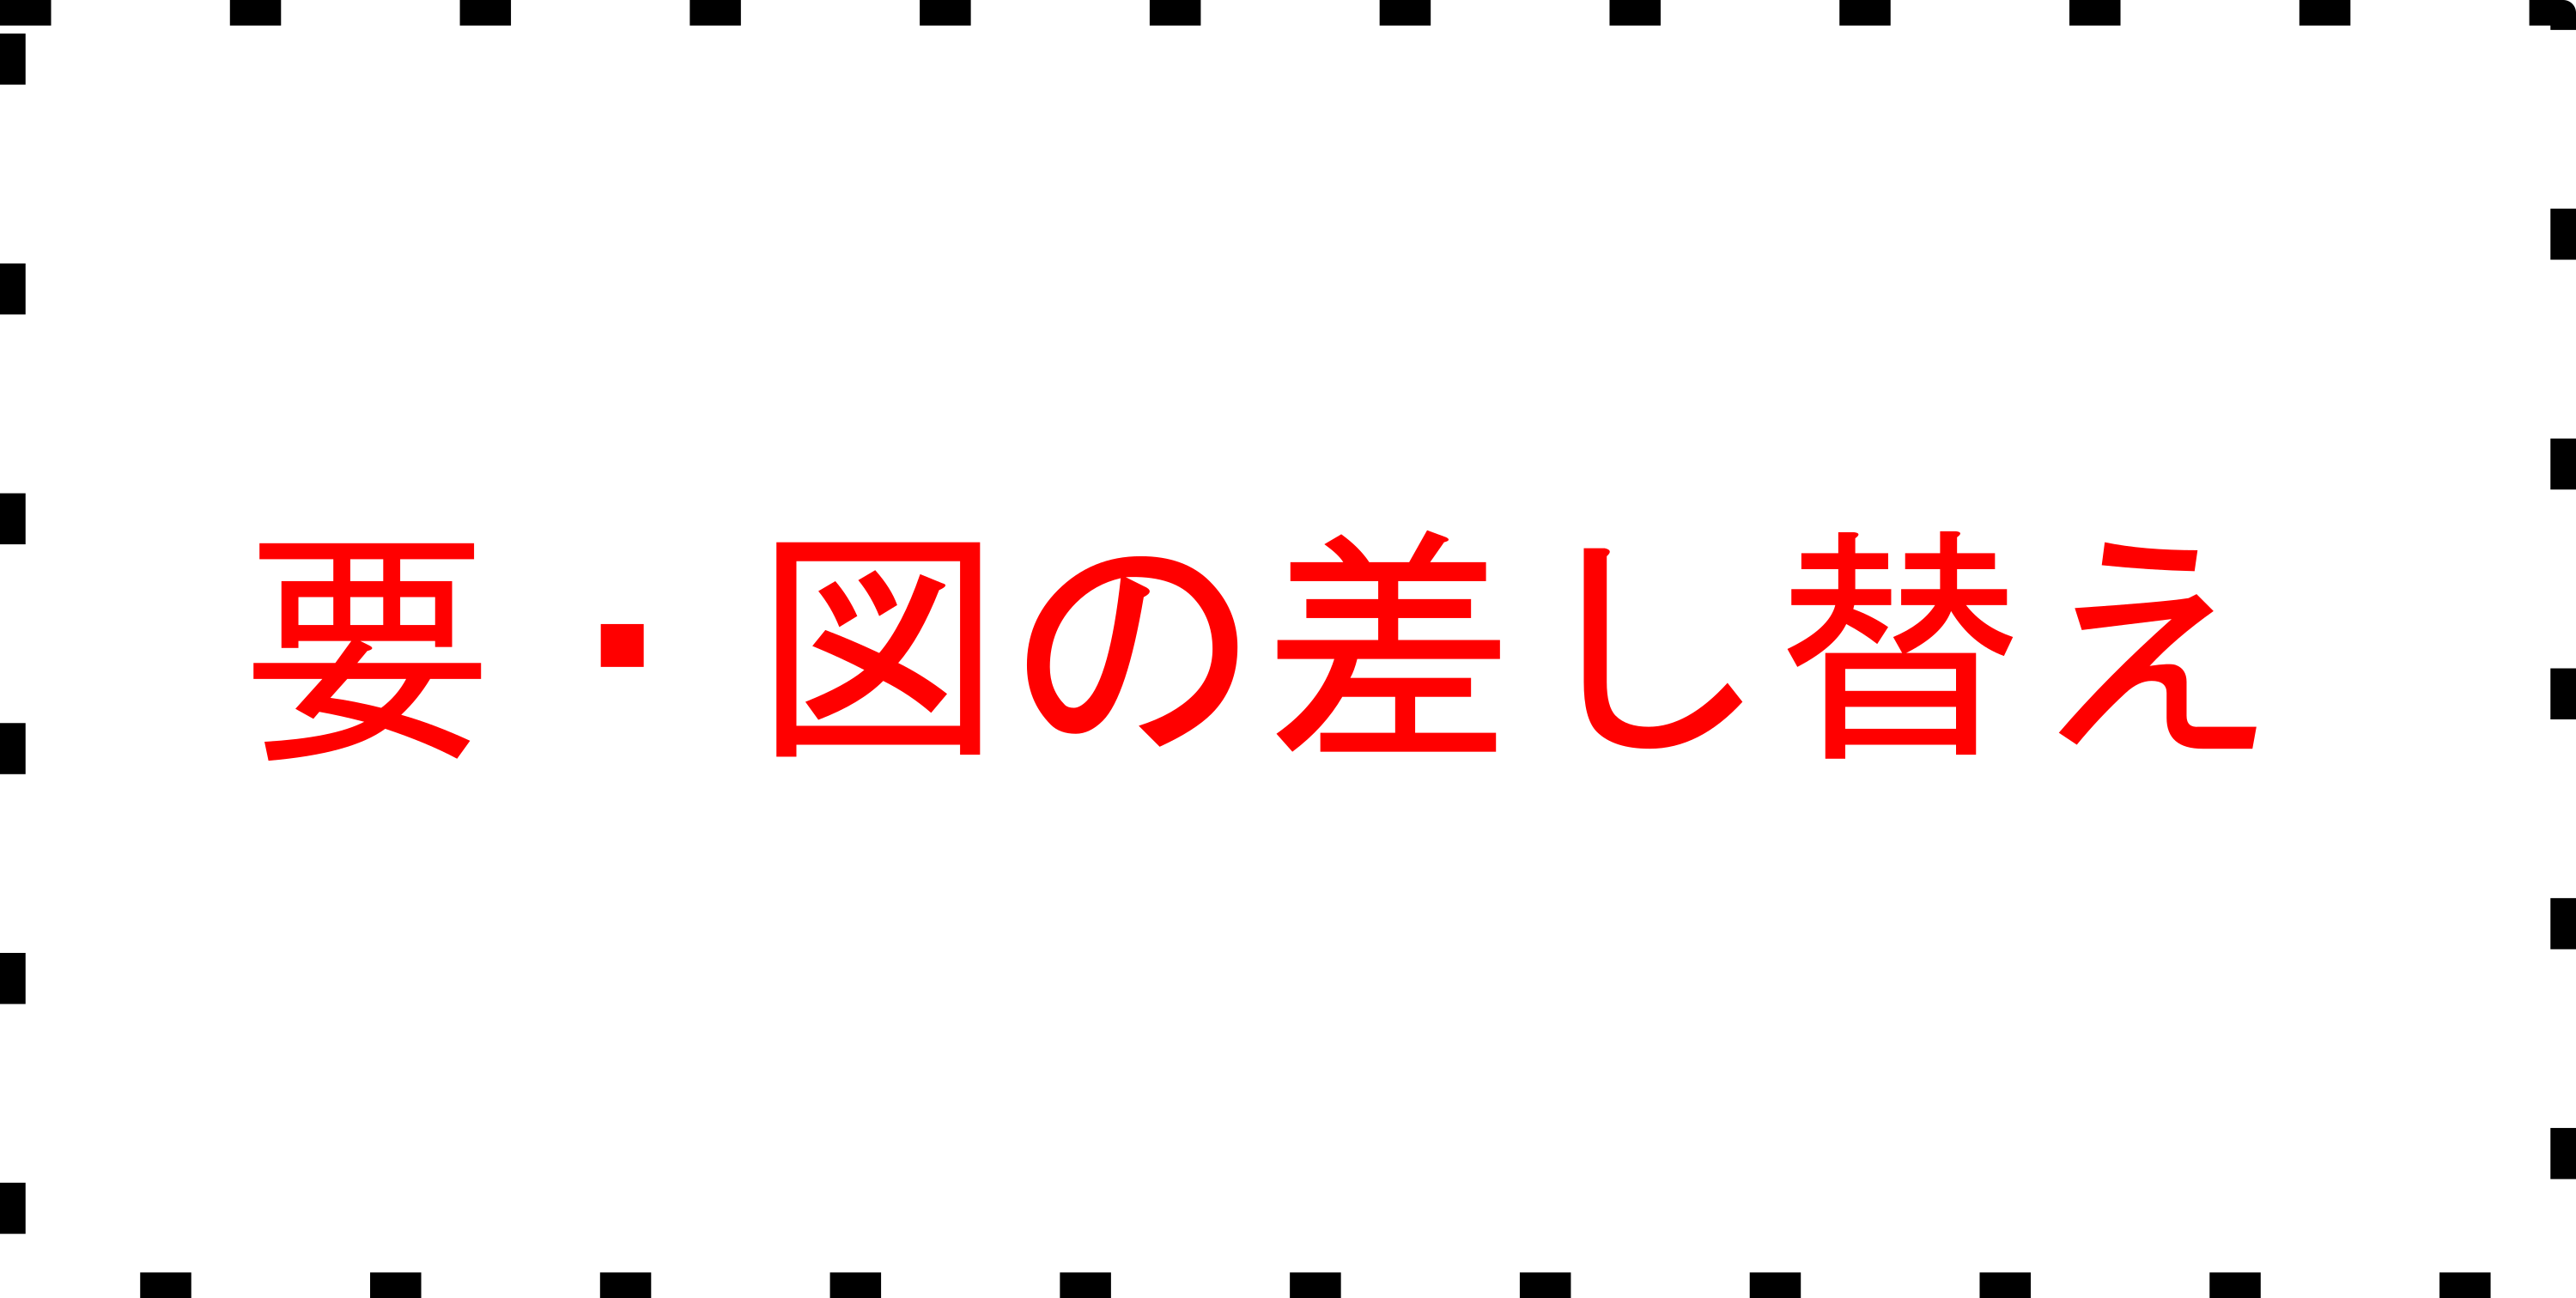
\includegraphics[width=10cm,clip]{tmp.png}
    \caption{Flow curve for 1wt.\%PAA solution. (After 1weeks)}
    \label{fig:PAA-vis}
\end{figure}

\section{圧力場 計測結果}

圧力場の計測を行った結果を

\begin{figure}
    \centering
    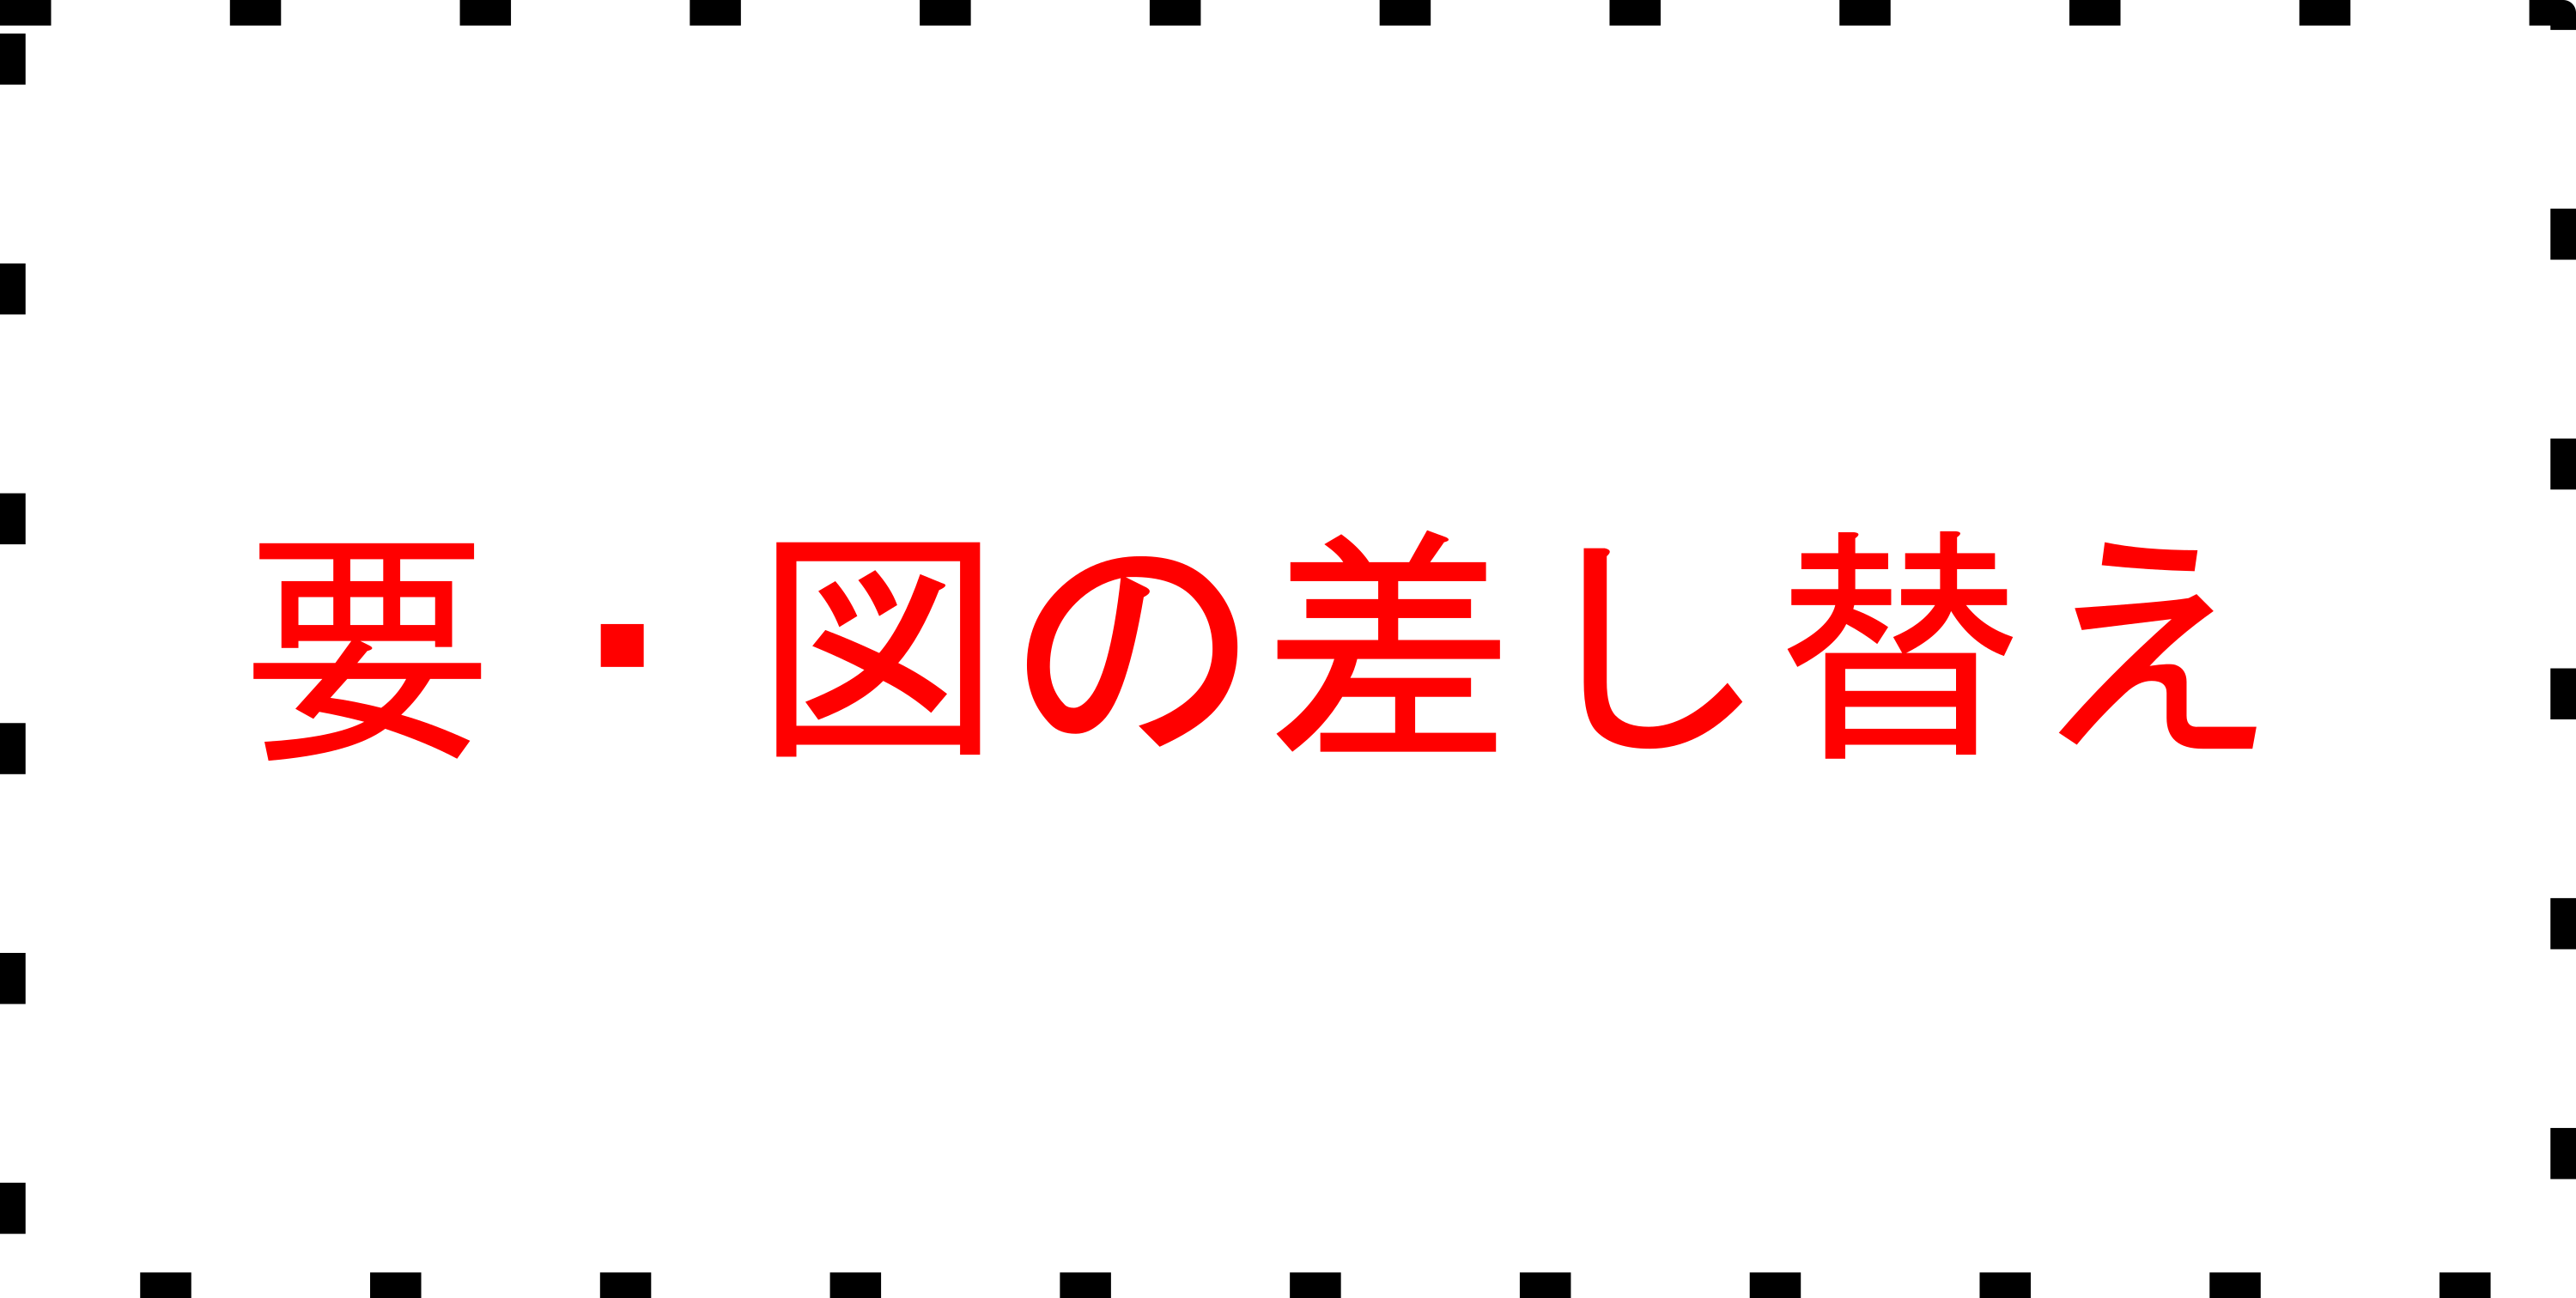
\includegraphics[width=10cm,clip]{tmp.png}
    \caption{Pressure field measurement results.}
    \label{fig:pressure}
\end{figure}

\section{落下球実験結果}

\begin{figure}[h]
    \centering
    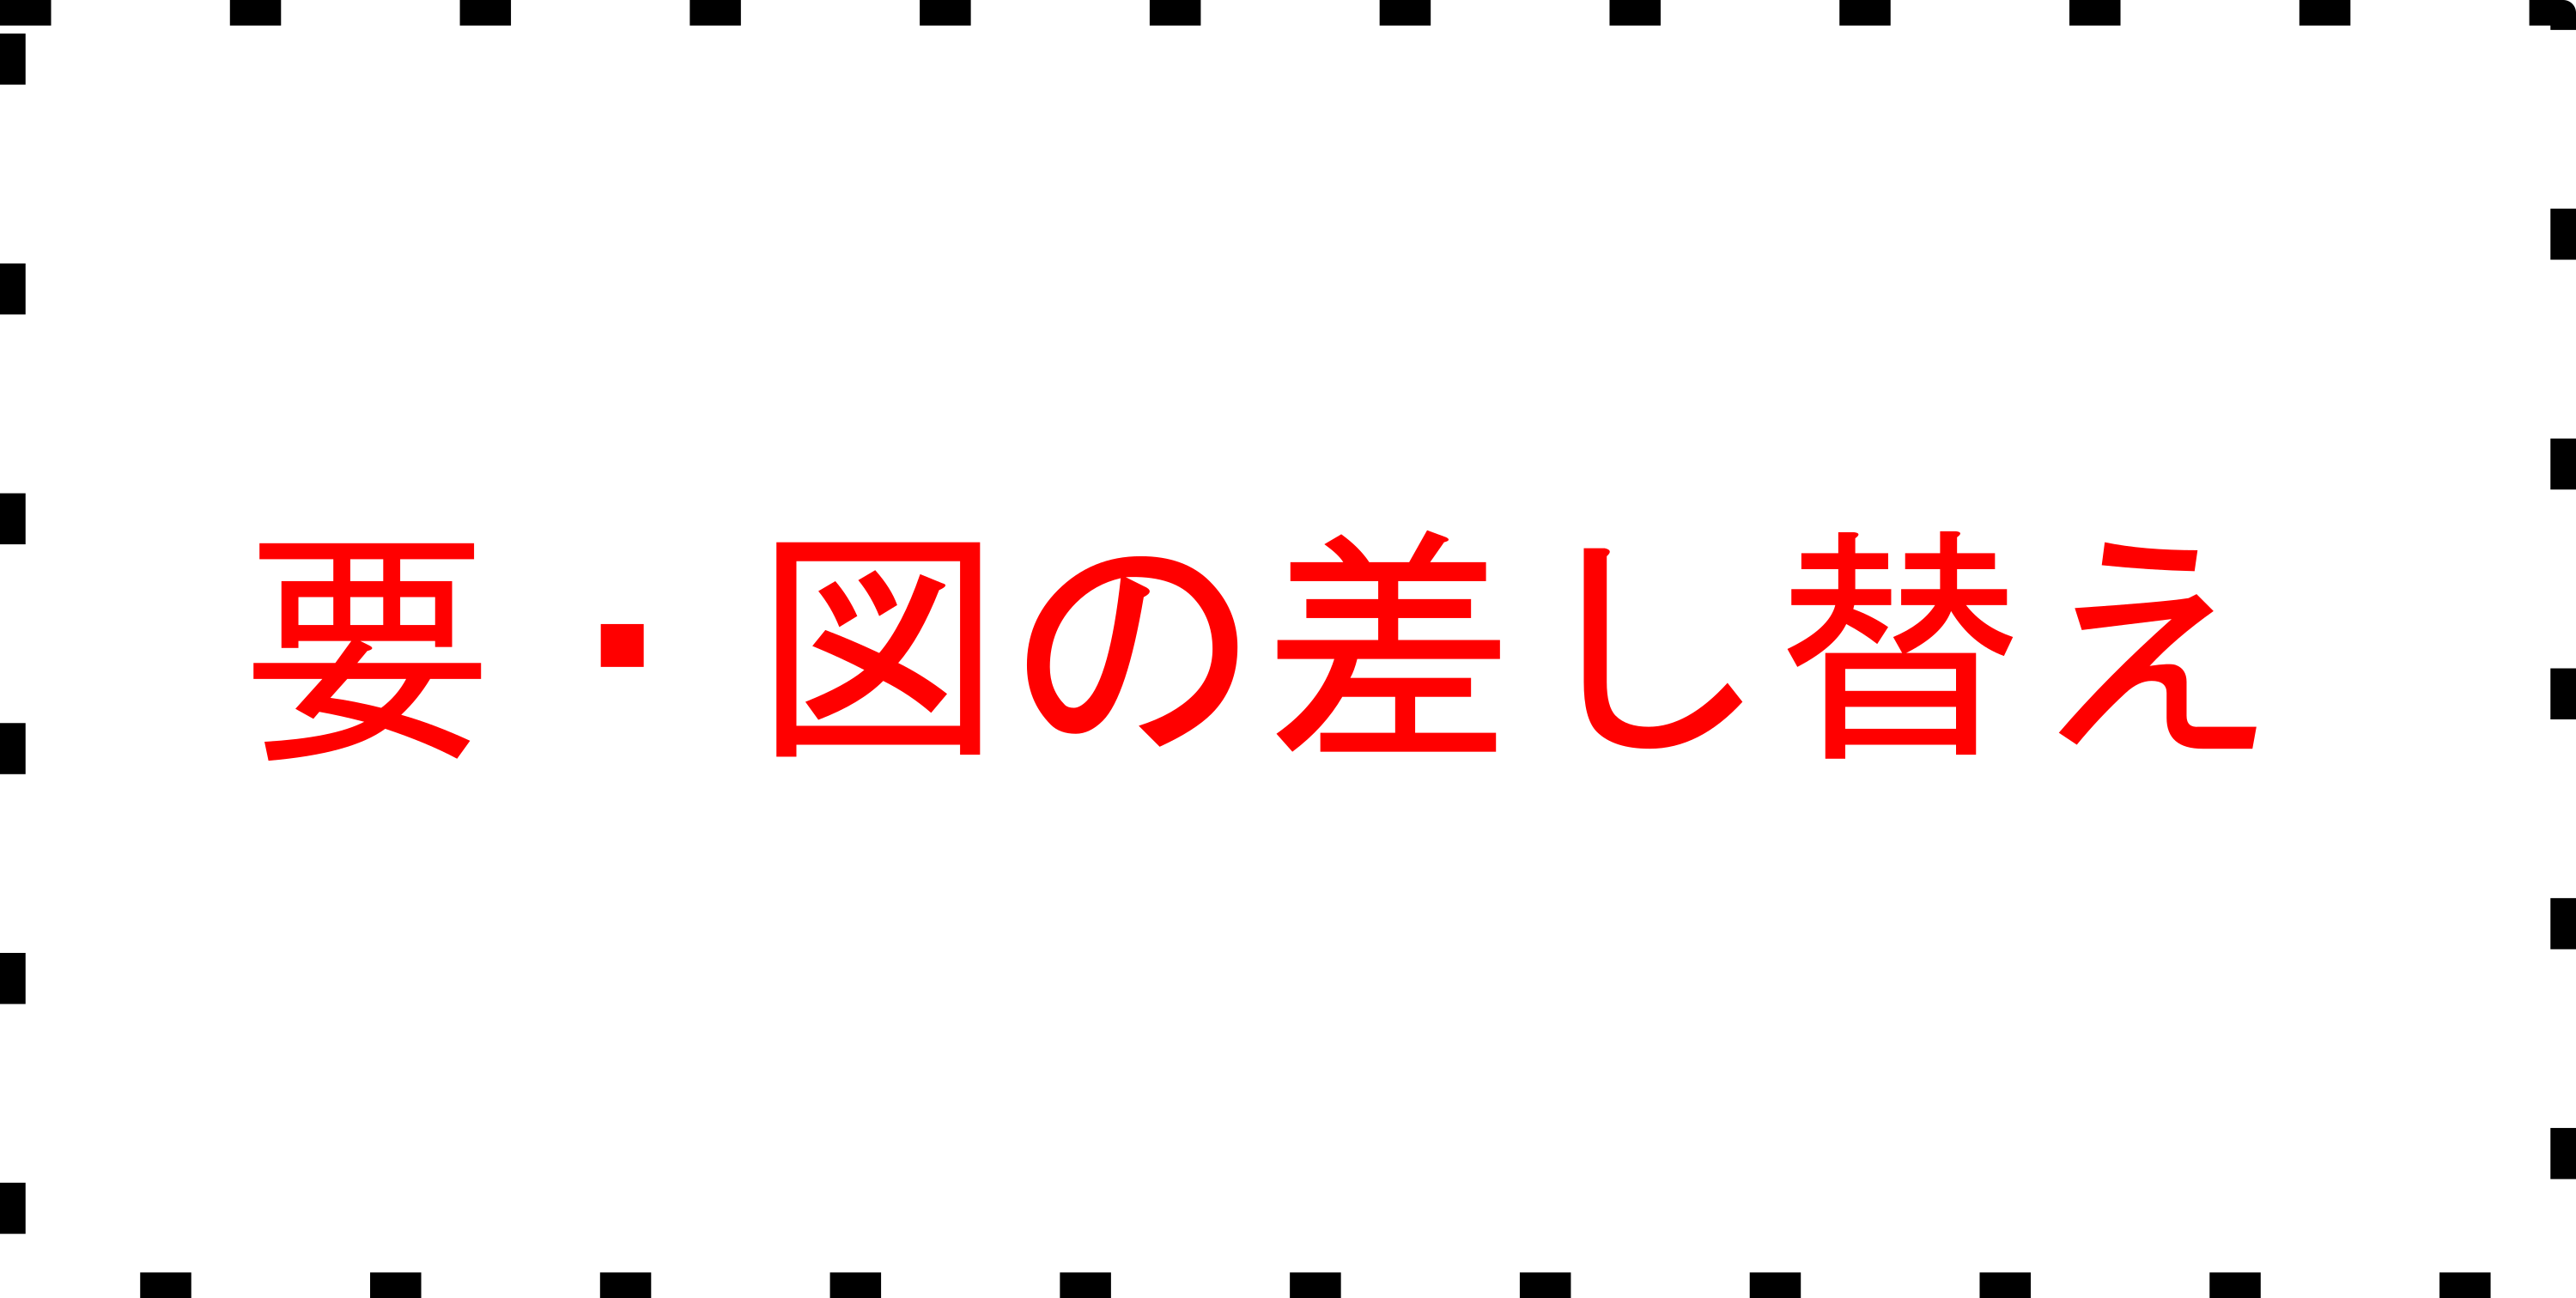
\includegraphics[width=10cm,clip]{tmp.png}
    \caption{Velocity of a falling sphere with a diameter of 2.4mm in water with or without ultrasound irradiation.}
    \label{fig:water}
\end{figure}

\begin{figure}[h]
    \centering
    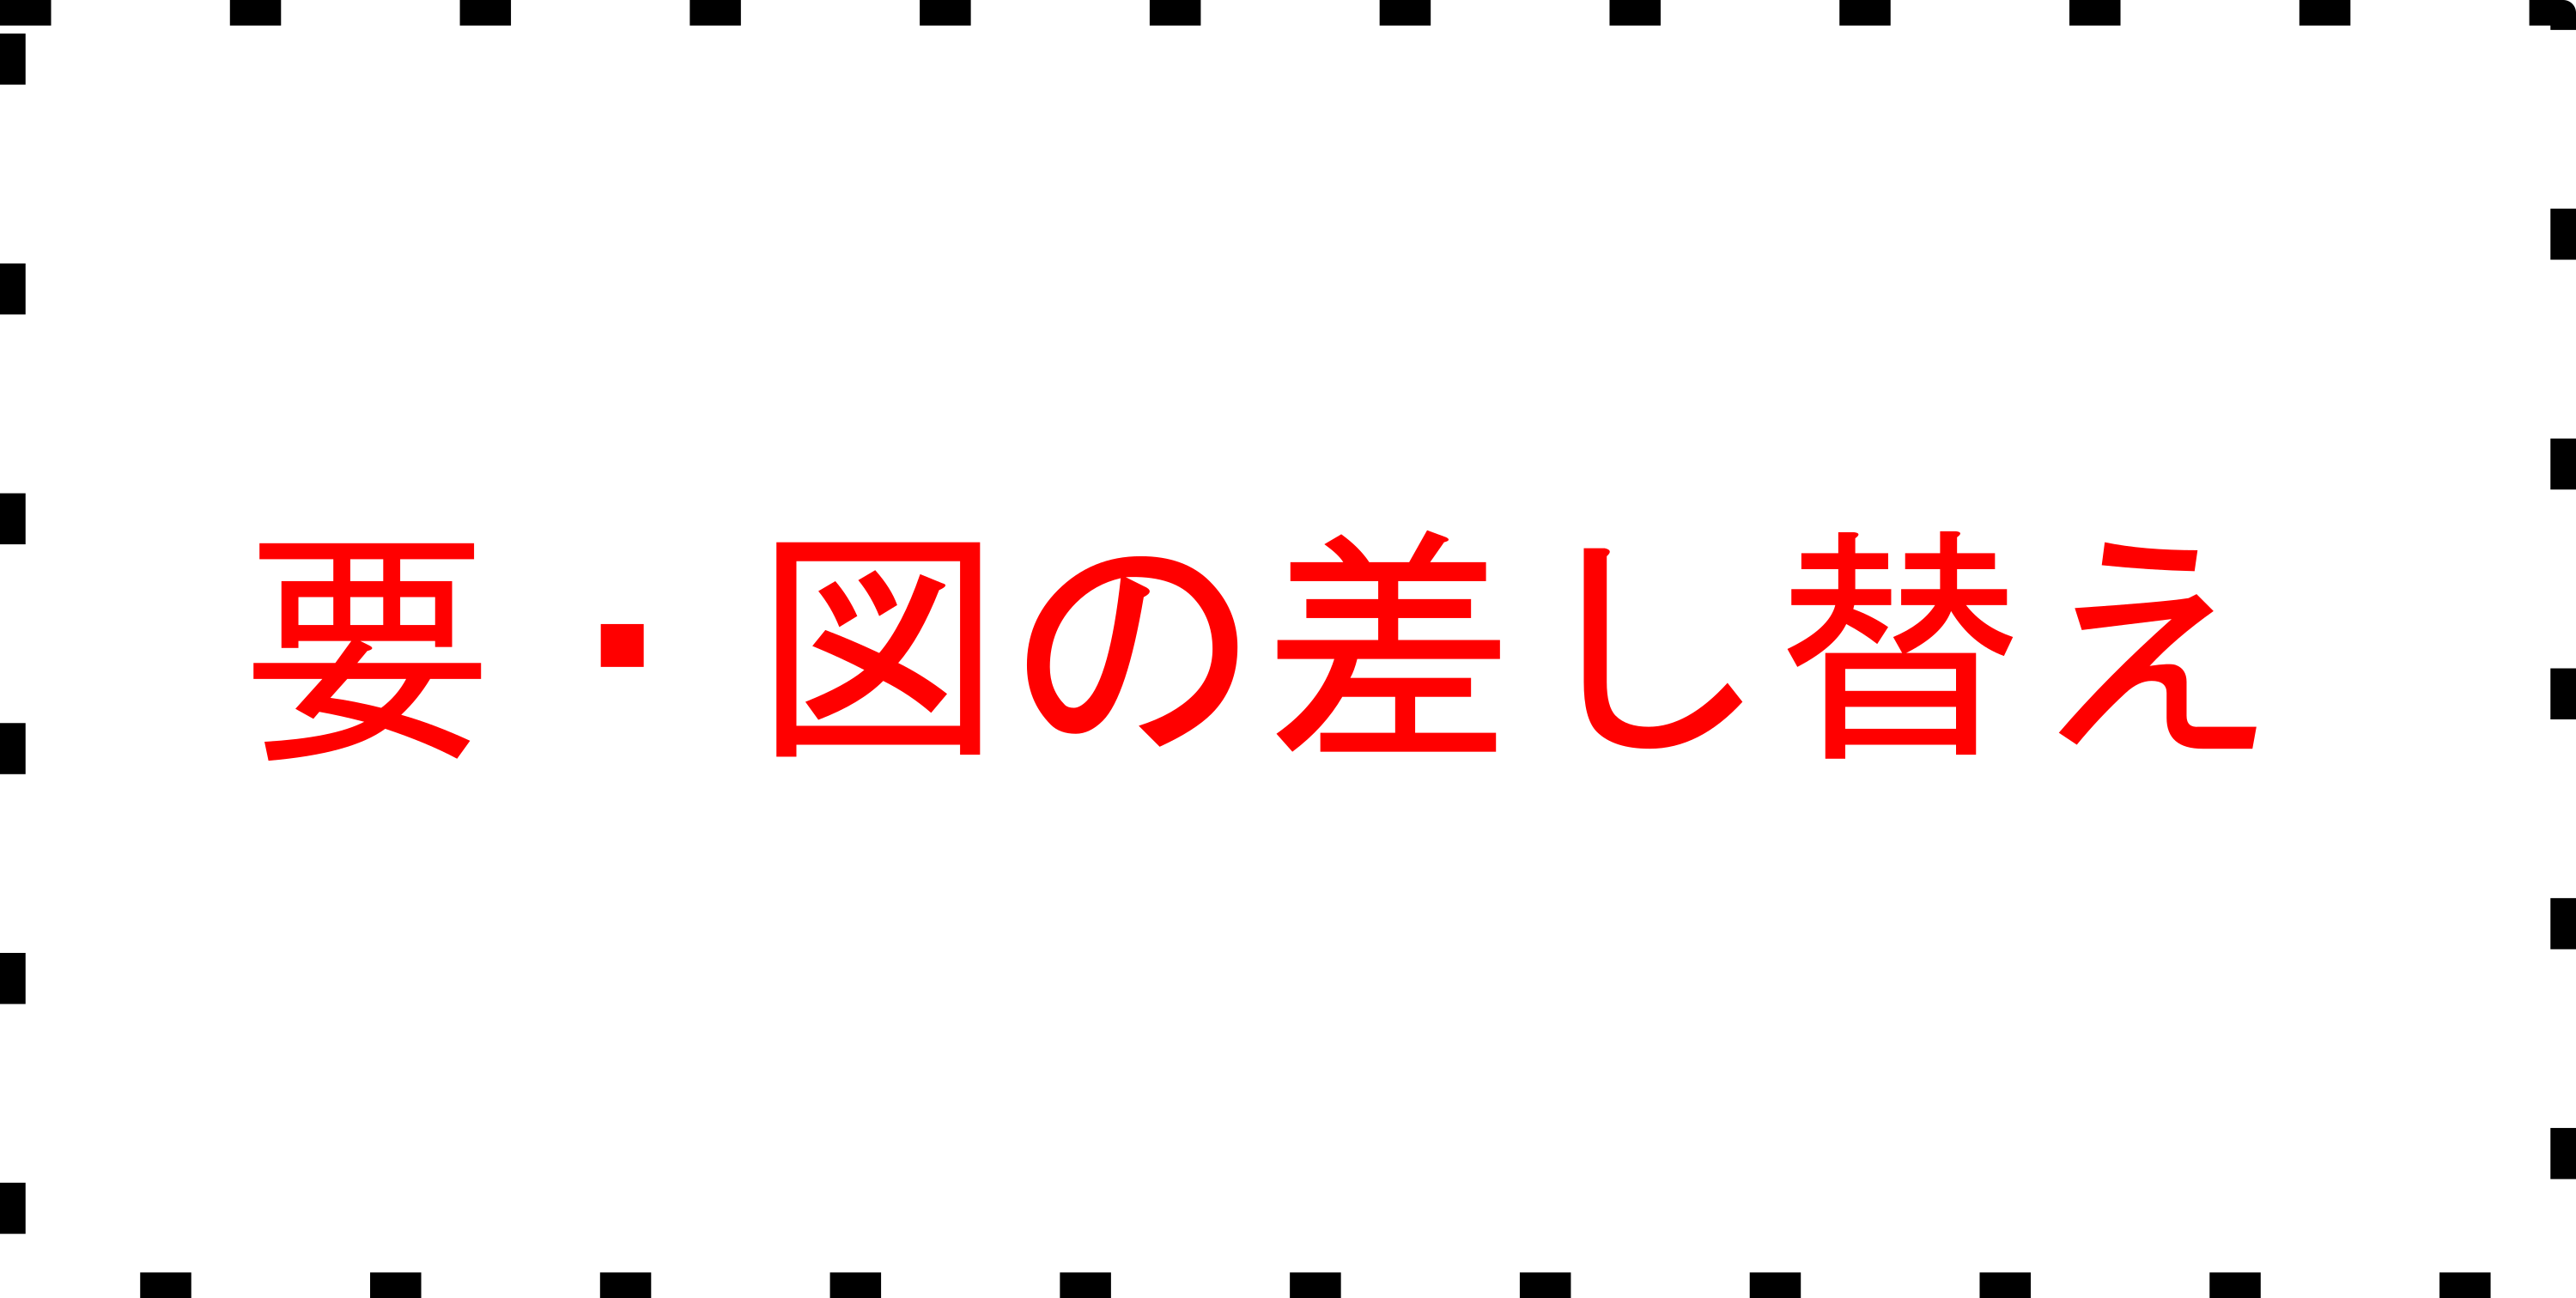
\includegraphics[width=10cm,clip]{tmp.png}
    \caption{Velocity of a falling sphere in PAA solution for various frequency of
        ultrasound irradiation.}
    \label{fig:PAA-falling}
\end{figure}
